\chapter{Estudo de Caso} \label{cap:estudodecaso}
Com o intuito de comparar o desenvolvimento de aplicações móveis utilizando a abordagem nativa e multiplataforma, 
foi realizado um estudo de caso. Para isso, um aplicativo feito em iOS 
nativo foi recriado utilizando o \textit{framework} Ionic. A seguir o aplicativo escolhido é detalhado em termos de funcionalidades e recursos utilizados. 

\section{Descrição do projeto selecionado} \label{sec:descricaodoprojeto}

Mini Farma é um aplicativo criado inicialmente para a plataforma iOS que serve para controle dos medicamentos que as 
pessoas possuem em casa em suas ``farmacinhas'' particulares.

\begin{figure}[h]
  \centering
    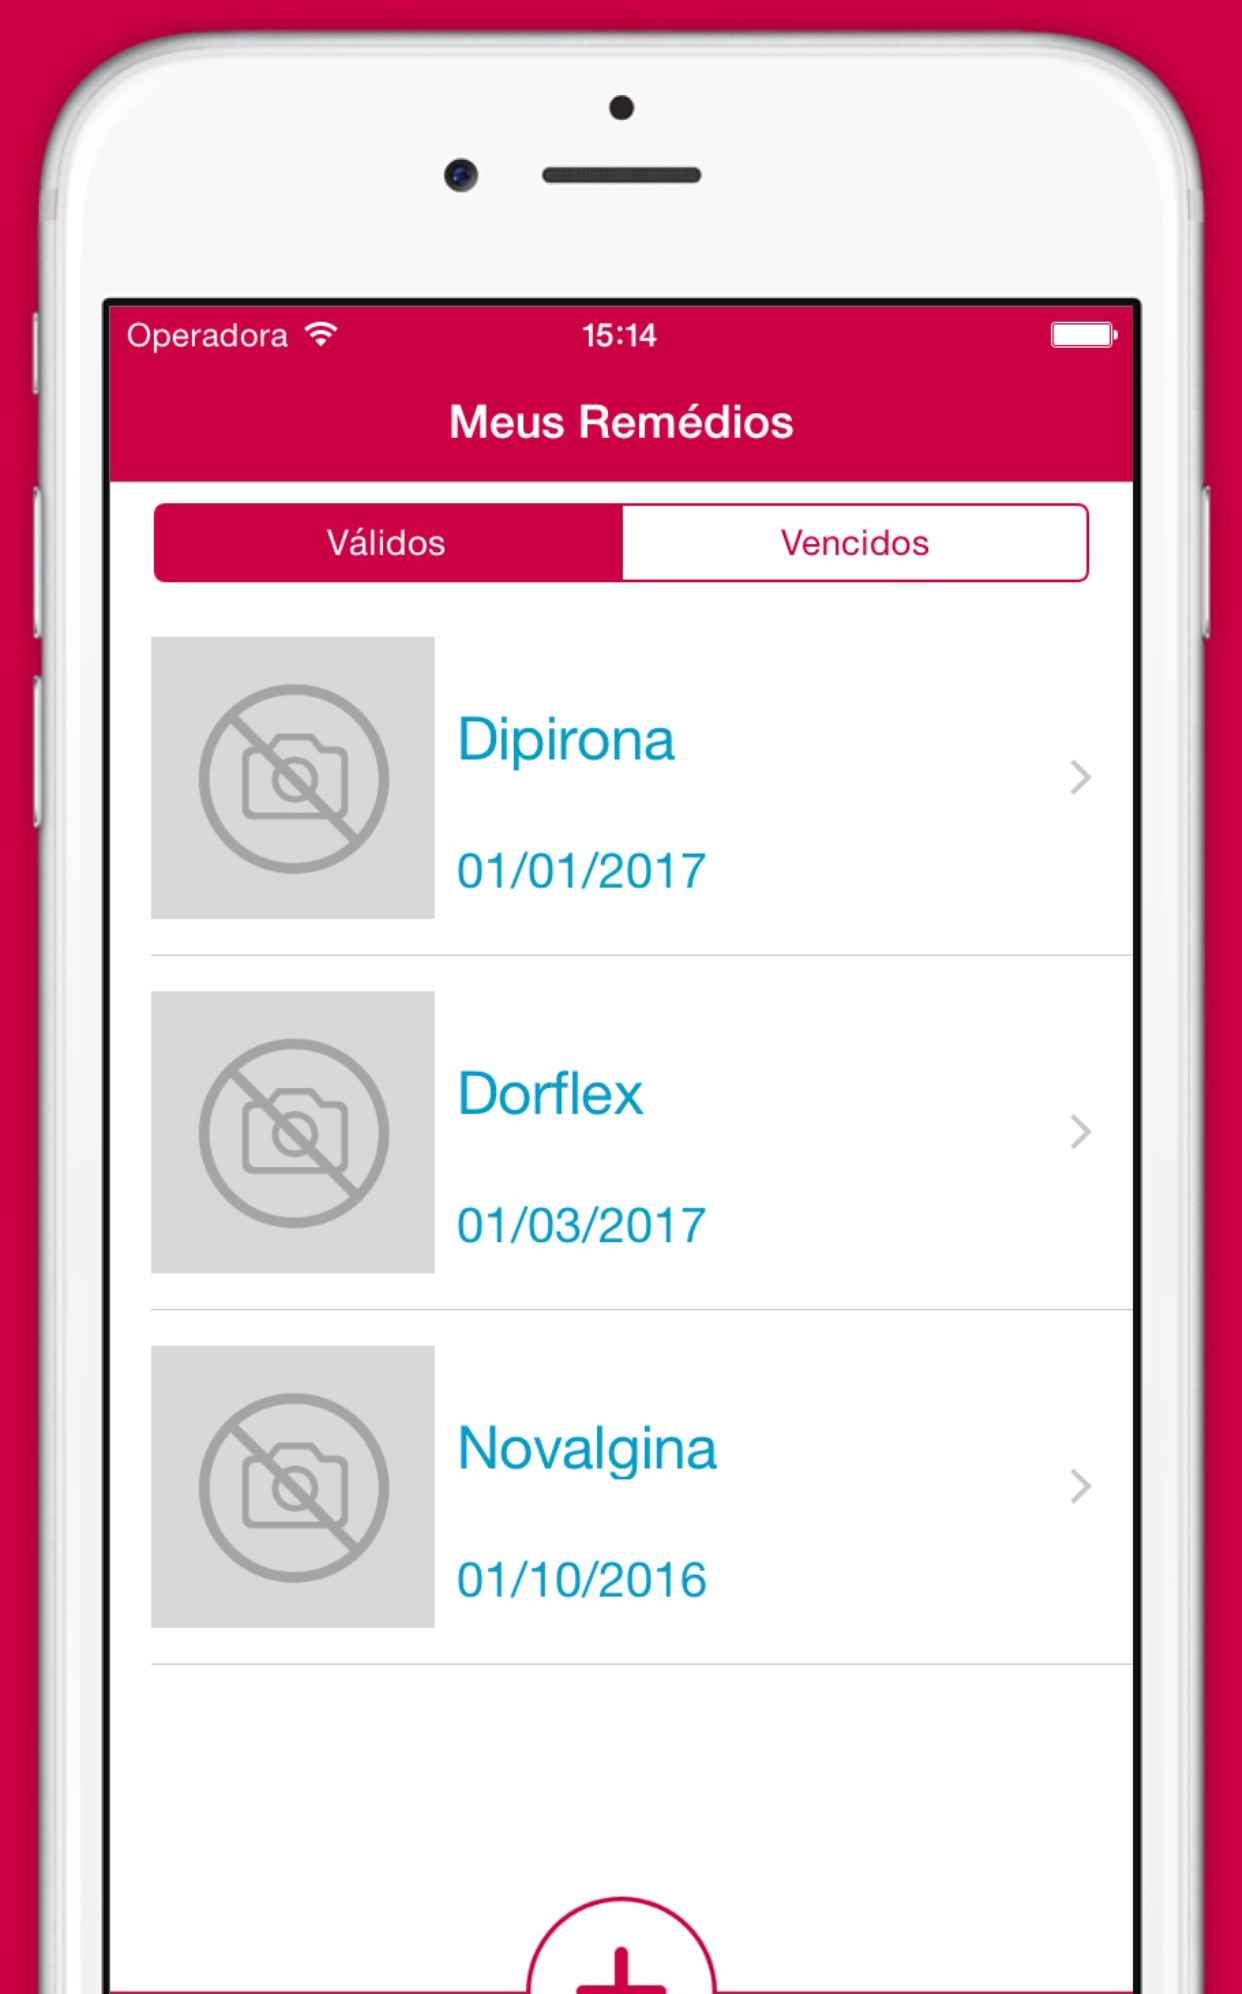
\includegraphics[width=0.5\textwidth]{minifarma}
    \caption[Tela inicial do aplicativo Mini Farma]{ Tela inicial do aplicativo Mini Farma. Fonte: Elaborado pelos autores.}
	\label{fig:minifarma}
\end{figure}

O aplicativo utiliza recursos nativos do sistema, os quais são descritos a seguir. 
\begin{itemize}
	\item \textbf{Localização geográfica}: Define a posição geográfica do dispositivo que o usuário está utilizando para salvar a 
    localização da farmácia onde ele comprou um medicamento para, caso seja necessário, explicar para alguém onde a 
    farmácia fica. Também é possível com base nessa localização da farmácia e do usuário, traçar uma rota para levá-lo diretamente à 
    farmácia em questão;
	\item \textbf{Notificações locais}: Diferente das notificações \textit{Push} as notificações locais são criadas e agendadas na central 
    de notificações do dispositivo e o sistema se encarrega de entregá-las corretamente de acordo com parâmentros definidos pelo aplicativo. 
    No caso do Mini Farma, as notificações são usadas para lembrar o usuário, na data e hora corretas, de que o mesmo deve tomar seus medicamentos;
	\item \textbf{Ligação}: As notificações podem conter ações que executam um determinado bloco de código dentro do aplicativo. No Mini Farma, 
    uma das notificações possíveis é a de aviso de pouca quantidade ou remédio esgotado, no caso do medicamento ter acabado. 
    Quando essa notificação é enviada, pode ser feita uma ligação diretamente pela ação da notificação para o número da 
    farmácia cadastrado no aplicativo. Dessa forma, o usuário pode solicitar uma nova quantidade de medicamento diretamente com a farmácia. 
	\item \textbf{Câmera}: Para facilitar a identificação dos medicamentos, é possível tirar uma foto com a câmera do dispositivo para 
    cada remédio cadastrado. Além de uma foto para o medicamento em si, é possível tirar uma foto da receita dele, caso haja;
    \item \textbf{Rolo de câmera}: Se o usuário já tiver uma foto que o ajude a identificar o seu medicamento ou da receita do mesmo salva 
    no rolo de câmera, é possível escolher a foto sem precisar tirar uma nova;
\end{itemize}

\textit{* Vale ressaltar, que com excessão da Ligação, todos os outros recursos nativos do sistema, precisam necessariamente serem autorizados pelo
usuário para funcionar. Caso o usuário não autorize, o aplicativo ficará com funcionalidades reduzidas.} 

Como banco de dados foi usado o SQLite, por meio do \textit{framework} externo e \textit{open-source FMDB}, 
disponível no \href{https://github.com/ccgus/fmdb}{Github};

A arquitetura do sistema foi criada com base no padrão de projeto \textit{MVC}, possuindo uma camada \textit{DAO} para comunicação 
com o banco de dados. No entanto, o \textit{MVC} tradicional difere em alguns aspectos do \textit{MVC} usado no iOS. 

No iOS o \textit{MVC} trás uma controladora ligada à classe de \textit{view}, que é chamado de \textit{ViewController}, que é responsável por 
criar a ponte entre a interação do usuário pela \textit{view} com as classes modelos. Dessa forma, as \textit{ViewControllers} têm a 
responsabilidade de repassar as entradas do usuário para a modelo e controlar a \textit{view} para apresentar os resultados que a modelo retornar.

Diferente do \textit{MVC} tradicional, no qual a controladora apenas repassa as informações que estão entrando na fronteira da aplicação, 
as \textit{ViewControllers} têm, além dessa responsabilidade, também a responsabilidade de instanciar e gerenciar a \textit{view} no tocante
a organização dos elementos e apresentação das informações.

Outra observação sobre as diferenças entre os dois \textit{MVCs}, é que no \textit{MVC} tradicional pode haver uma controladora apenas 
para todas as modelos ou uma controladora por modelo, mas nenhuma ligada diretamente a uma \textit{view}, no entanto, no iOS há uma 
\textit{ViewController} por \textit{view}, podendo haver ainda uma controladora relacionada com cada modelo conforme o padrão tradicional do \textit{MVC}.

\begin{figure}[h]
  \centering
    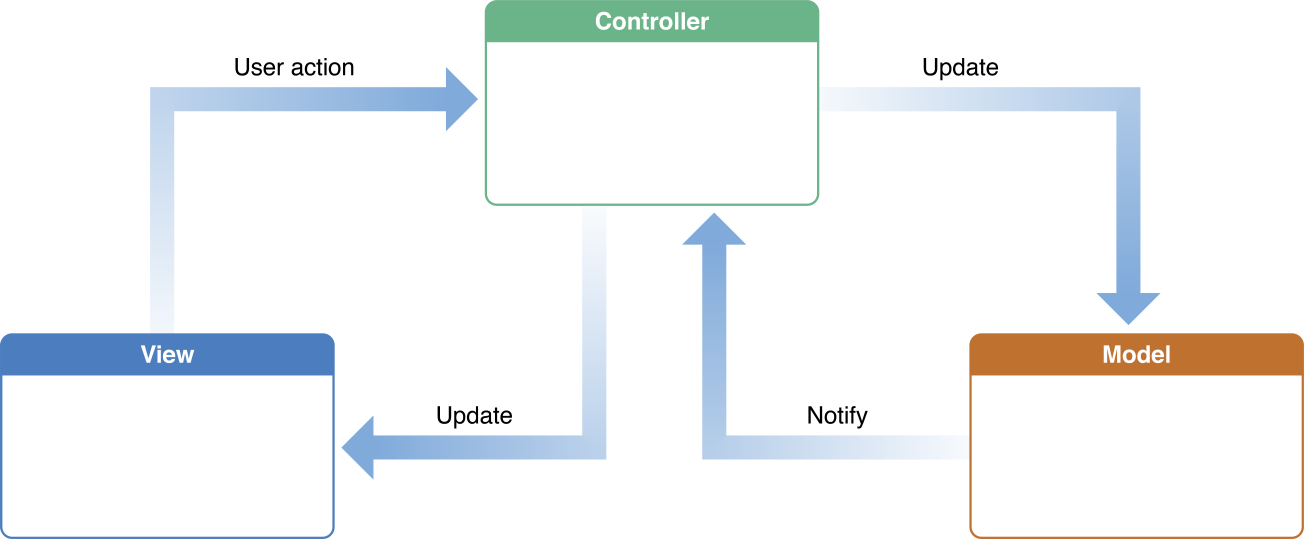
\includegraphics[width=1.0\textwidth]{mvc}
    \caption[Padrão \textit{Model-View-Controller}]{ Padrão \textit{Model-View-Controller}. Fonte: Apple Documentation.}
	\label{fig:mvc}
\end{figure}

\subsection{Ambiente de desenvolvimento} \label{subsec:ambientedesenvolvimento}
Nesta seção é apresentado todo o ambiente de desenvolvimento do \textit{app} Mini Farma quando foi feito originalmente para a plataforma iOS. 
O projeto foi executado contando com uma equipe de dois integrantes com conhecimentos intermediários na plataforma iOS. 
Os detalhes técnicos são listados a seguir.
\begin{itemize}
    \item \textbf{Máquinas}: Dois MacBook Pro Retina 13", processador \textit{Intel Core i5}, 8 GB de \textit{RAM};
    \item \textbf{Sistema Operacional das máquinas}: \textit{Mac OS X Yosemite} v10.10.5;
    \item \textbf{Sistema Operacional alvo do aplicativo}: iOS 8;
    \item \textbf{\textit{IDE}}: \textit{Xcode} v6.4;
    \item \textbf{Linguagem de Programação}: \textit{Swift} v1.3;
    \item \textbf{Banco de dados}: SQLite v3.8.10.2;
    \item \textbf{Ambiente de suporte}: \textit{Plugin SQLite Manager} para \textit{Mozilla Firefox}, para criação do banco de dados;
\end{itemize}

\section{Desenvolvimento multiplataformas do projeto} \label{sec:desenvolvimentomulti}

A partir do aplicativo feito em iOS, foi construída uma versão utilizando o Ionic para as plataformas Android e iOS.
Para a criação dessa versão do \textit{app}, a equipe foi alterada, mas permaneceu com dois integrantes, que são os autores deste trabalho.
No entanto, os integrantes não possuíam qualquer conhecimento prévio nos \textit{frameworks} Ionic, AngularJS e Cordova
e apenas possuíam um conhecimento básico em \textit{HTML}, \textit{CSS} e \textit{JavaScript}. Os detalhes técnicos são listados a seguir.
   
\begin{itemize}
    \item \textbf{Máquinas}: Dois MacBook Pro Retina 13", processador \textit{Intel Core i5}, 8 GB de \textit{RAM};
    \item \textbf{Sistema Operacional das máquinas}: \textit{Mac OS X El Capitan} v10.11.5;
    \item \textbf{Sistema Operacional alvo do aplicativo}: iOS 9.3 e Android 6.0.0;
    \item \textbf{\textit{IDE}}: \textit{WebStorm} v2016.1.1;
    \item \textbf{\textit{Frameworks}}:
    \begin{itemize}
        \item \textbf{Ionic}: \textit{Copenhagen} v1.2.4*;
        \item \textbf{AngularJS}: \textit{foam-acceleration} v1.4.3*;
        
        * Durante a execução deste trabalho, já haviam sido disponibilizadas as versões 2 do Ionic e do AngularJS, no entanto,
        os autores optaram por não utilizá-las por ainda se tratarem de versões \textit{beta} e portanto instáveis, o que poderia 
        impactar negativamente no desenvolvimento do projeto.
        
        \item \textbf{Cordova}: v6.0.0;
    \end{itemize}
    \item \textbf{Linguagem de Programação}: \textit{JavaScript} v1.7. 
    \begin{itemize}
        \item \textit{HTML} 5 e \textit{CSS} 3 foram usados paralelamente para a criação da interface gráfica do aplicativo;
    \end{itemize}
    \item \textbf{Banco de dados}: SQLite v3.8.10.2;
    \item \textbf{Ambiente de suporte}: Google Chrome, para \textit{debug} do aplicativo;
    \item \textbf{Simuladores}: 
    \begin{itemize}
        \item \textbf{iOS}: iPhone 6S Plus
        \item \textbf{Android}: Nexus 7
    \end{itemize}
\end{itemize}

\subsection{Relato de desenvolvimento} \label{subsec:experienciasdev}

É apresentado, a seguir, o relato das experiências obtidas durante o desenvolvimento com Ionic, divido nas funcionalidades 
já descritas na Subseção~\ref{subsection:planejamentodesenvolvimento} deste trabalho, bem como feita a comparação entre o desenvolvimento nativo para iOS e 
o multiplataforma Ionic. Há, ainda, um tópico de observações gerais pertinentes à implementação do \textit{app} como um todo. 


 \begin{itemize}
 	
 	\item \textbf{Listagem de Remédios e Alertas};
		\begin{itemize}
			\item Para a tela inicial do \textit{app}, a lista de remédios e alertas, foi preciso realizar uma pequena alteração em relação ao original, para considerar, agora, 
			dois sistemas operacionais diferentes (iOS e Android). Foi preciso criar duas 
			\textit{views} para a mesma tela, pois o componente de abas (conhecido como \textit{tabs}), é diferente no iOS e no Android. Com isso, quando foi feito pensando-se no iOS do Ionic, ele não correspondia 
			muito bem ao padrão de interface do Android, por isso foi preciso criar duas telas separadas e fazer uma verificação se o dispositivo é iOS ou Android. Após feita a verificação de dispositivo, o próprio
			Ionic se encarrega de definir a aparência do componente para o padrão do sistema no qual o aplicativo está sendo executado.

			\item Para a criação da lista de remédios e alertas que o usuário possui cadastrados, o componente usado no iOS é chamado de \textit{UITableView}. No Ionic, o componente similar é o conjunto das diretivas 
			\textit{ion-list} e \textit{ion-item} do Ionic com a diretiva \textit{ng-repeat} do AngularJS. 
			É muito simples de ser implementada, possuindo documentação ampla e exemplos de uso nos \textit{sites} oficiais dos \textit{frameworks}.

			\item Para a realização das filtragens dos remédios por data de validade, e dos alertas por ativos e inativos, bastou usar o componente \textit{filter} padrão do AngularJS. Dessa forma, foi possível 
			mostrar apenas as informações que deveriam ser mostradas. Novamente, possuindo muitos exemplos e ajuda na documentação do \textit{framework}.

			 \begin{figure}[H]
			 	\centering
			 	\begin{minipage}{.5\textwidth}
			 		\centering
			 		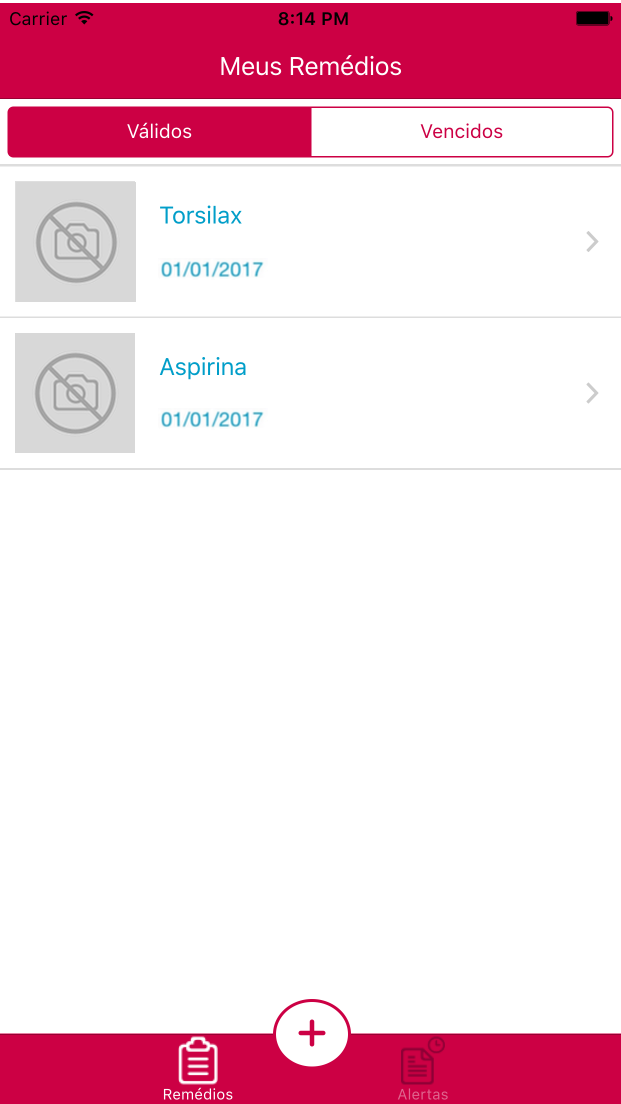
\includegraphics[width=.8\linewidth]{ionic_lista_ios}
			 	\end{minipage}%
			 	\begin{minipage}{.5\textwidth}
			 		\centering
			 		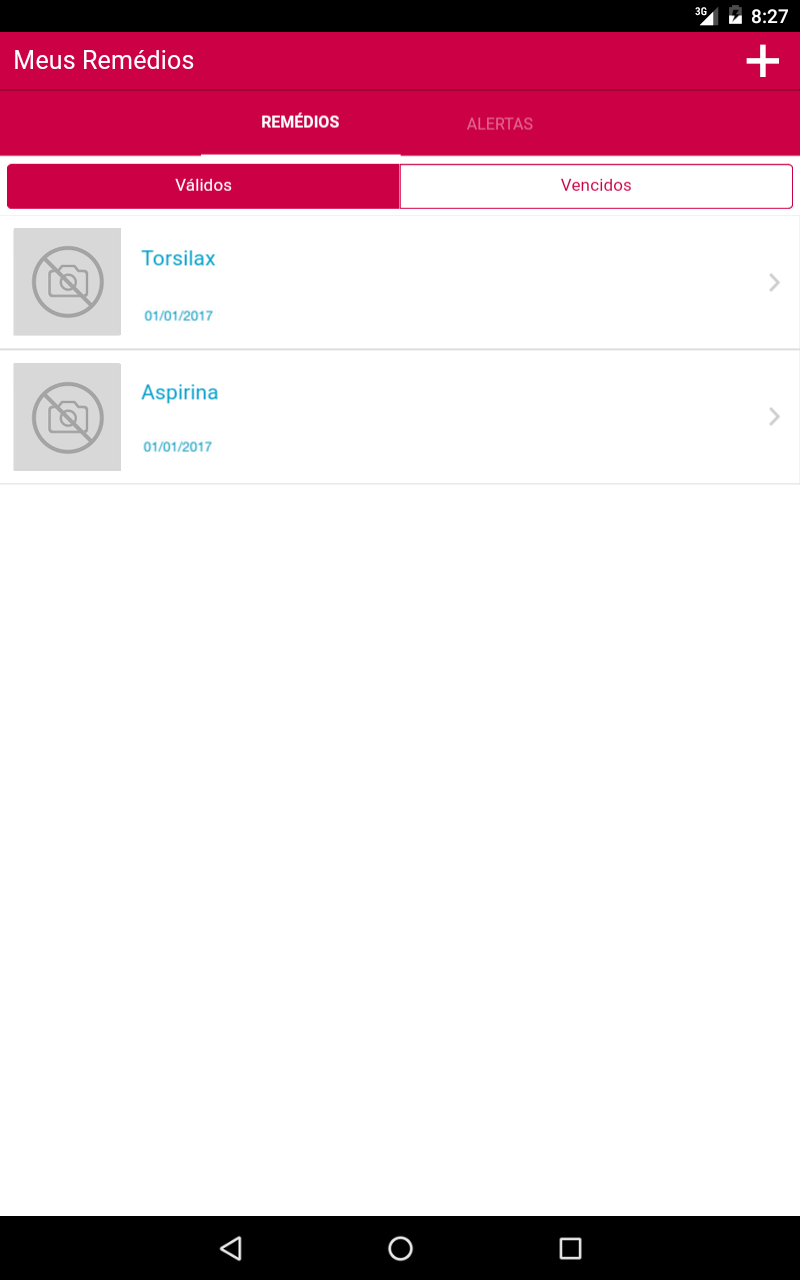
\includegraphics[width=0.9\linewidth]{ionic_lista_android}
			 	\end{minipage}
			 	\caption[Telas da lista de remédios (iOS \textit{versus} Android)]{ Telas da lista de remédios (iOS \textit{versus} Android). Fonte: Elaborado pelos autores.}
			 	\label{fig:ionic_lista}
			 \end{figure}

		\end{itemize}

 	\item \textbf{Cadastro de Remédios};
 	
 		 \begin{itemize}
			\item No cadastro de remédios há o uso da câmera do dispositivo para tirar uma foto do medicamento e para registrar a prescrição médica. Opcionalmente, pode-se selecionar as fotos a partir da biblioteca de imagens do dispositivo. Com o uso do \textit{plugin} Cordova de acesso à câmera, essa foi uma tarefa tranquila e que funcionou corretamente em ambas as plataformas, Android e iOS. 
			\item Para que o usuário opte entre  tirar uma nova foto e escolher da galeria do dispositivo, foi utilizado um componente conhecido no iOS como \textit{UIActionSheet}. Com o uso de um único código, o Ionic possibilitou a geração de um componente exatamente igual ao nativo do iOS e de um correspondente no Android. 
			Na Figura~\ref{fig:ionic_action_camera} é possível observar as diferenças de interface, as quais foram adequadas pelo Ionic para cada plataforma.
			
			 \begin{figure}
			 	\centering
			 	\begin{minipage}{.5\textwidth}
			 		\centering
			 		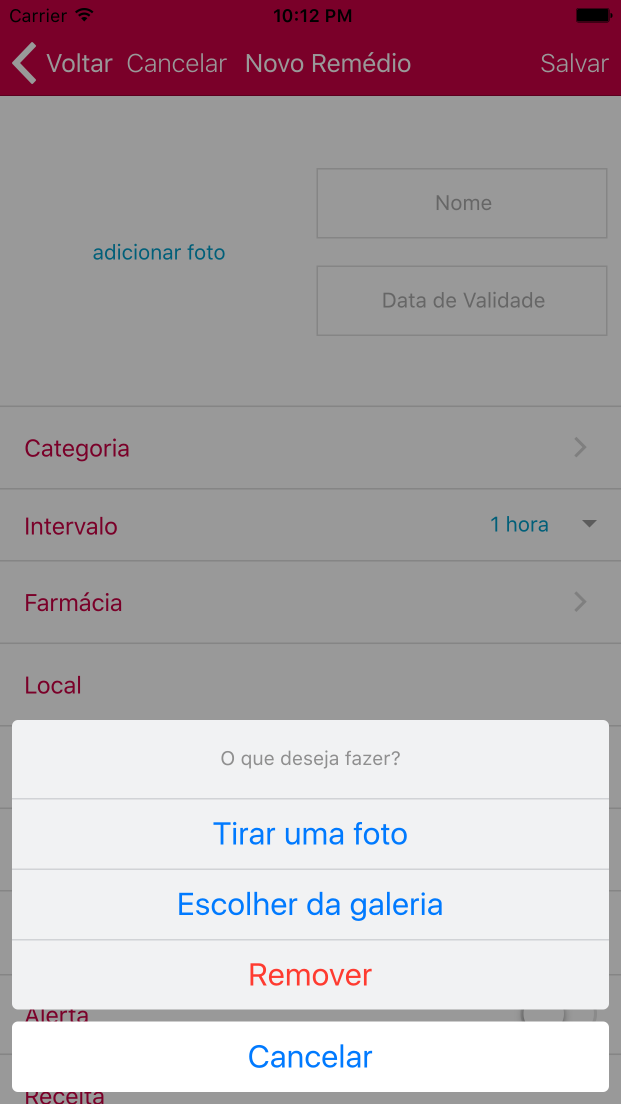
\includegraphics[width=.8\linewidth]{ionic_action_camera_ios}
			 	\end{minipage}%
			 	\begin{minipage}{.5\textwidth}
			 		\centering
			 		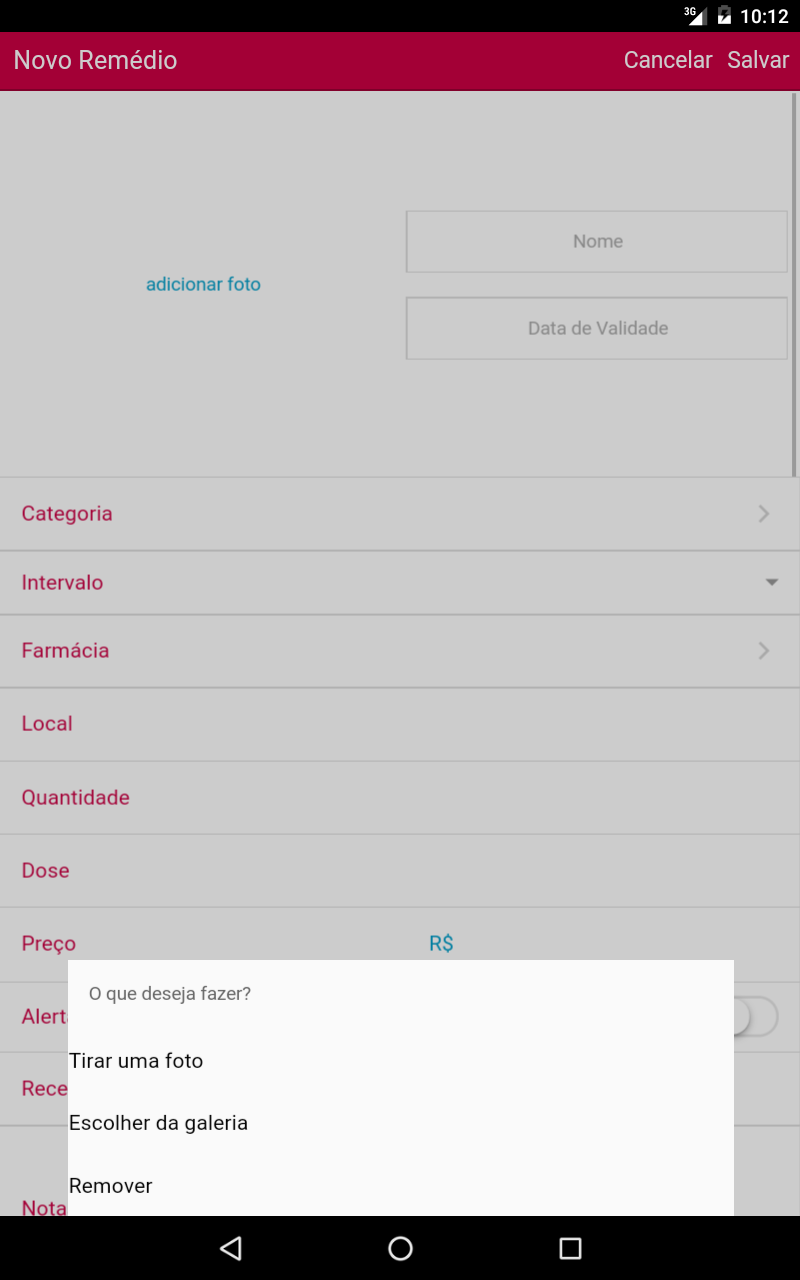
\includegraphics[width=0.9\linewidth]{ionic_action_camera_android}
			 	\end{minipage}
			 	\caption[Telas de cadastro de foto de remédio (iOS \textit{versus} Android)]{ Telas de cadastro de foto de remédio (iOS \textit{versus} Android). Fonte: Elaborado pelos autores.}
			 	\label{fig:ionic_action_camera}
			 \end{figure}
			 
			 	\item Para a criação de uma nova categoria de remédios, foi utilizada interação por meio de uma caixa de diálogo, também conhecido como alerta. Para isso, utilizou-se os chamados \textit{popups} do Ionic.  Apesar de facilmente implementados e personalizáveis, esses componentes não se assemelham às caixas de diálogo nativas do iOS, \textit{UIAlertView} e do Android, \textit{AlertDialog}. O alerta criado é apresentado na Figura~\ref{fig:ionic_alert}. Posteriormente,  foi verificado que há no Cordova uma \textit{API} para caixas de diálogo que, diferente da disponibilizada pelo Ionic, gera uma interface adequada aos padrões de ambas as plataformas. Um exemplo de alerta  gerado pelo Cordova e idêntico à uma das plataformas, neste caso o iOS, é apresentado na Figura~\ref{fig:ios_prompt}.
			 	
			 	\begin{figure}[H]
			 		\centering
			 		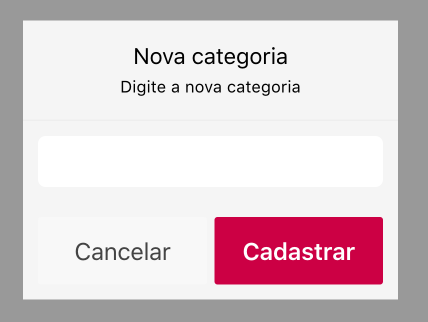
\includegraphics[width=0.5\textwidth]{ionic_alert}
			 		\caption[Tela de alerta]{Tela de alerta. Fonte: Elaborado pelos autores.}
			 		\label{fig:ionic_alert}
			 	\end{figure}
			 	
			 	\begin{figure}[H]
			 		\centering
			 		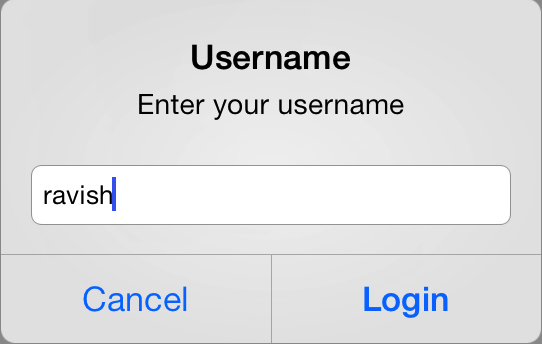
\includegraphics[width=0.5\textwidth]{ios_prompt}
			 		\caption[Alerta Cordova - iOS]{Alerta Cordova - iOS. Fonte: \cite{framework_ngcordova_2016}.}
			 		\label{fig:ios_prompt}
			 	\end{figure}
			 	
			 	\item Em relação ao banco de dados, utilizou-se a \textit{API} Cordova SQLite. Como o banco de dados construído nativamente também foi feito utilizando o SQLite, foi possível aproveitar os \textit{scripts} de definição e manipulação de dados. Não houveram complicações no uso da \textit{API} e facilmente foram encontrados exemplos de uso na internet que auxiliaram na estruturação da camada de comunicação do aplicativo com o banco de dados.
			 	
			 	\item picker view [foto comparando do de intervalo] (imendar no de action)
			 	
			 	\item {red}{passar dados de uma pagina para outra, semelhante ao protocolo do ios em questao de dificuldade} (tb usando no cadastro de alertas)
			 	
			 	\item celulas colapsaveis na tela de add remedio
			 	
			 	\item foto e comparar a selecao do local
			 	
			 	\item Visao geral do cadastro
			 	

			 
		 \end{itemize}
     \item \textbf{Cadastro de Farmácias}; 	
	 \begin{itemize}
		\item Para cadastrar uma nova farmácia, o usuário deve marcar no mapa onde a farmácia se encontra. Para a utilização do mapa no Ionic, foi utilizada a \textit{API Maps} do Google, diferentemente da 
		\textit{API MapKit} do iOS. Não houveram grandes dificuldades na criação do mapa e renderização do mesmo na tela. A dificuldade de implementação é similar a do iOS nativo.
		Apenas realizando pesquisas e estudos na documentação da \textit{API} do Google, 
		já foi possível a elaboração do que precisava ser feito, no caso, mostrar o mapa e fornecer a opção de mover o pino para um local específico e capturar as coordenadas daquele ponto. No caso, foi 
		necessário utilizar a diretiva \textit{map} para renderização do mapa na tela e definir o \textit{callback} de reposicionamento do cursor e captura da localização. Na Figura~\ref{fig:add_farma} é possível 
		ver as diferenças entre o mapa do \textit{MapKit} do iOS e da \textit{API Maps} do Google.
	 \end{itemize}
	 \begin{figure}[H]
		\centering
		\begin{minipage}{.5\textwidth}
			\centering
			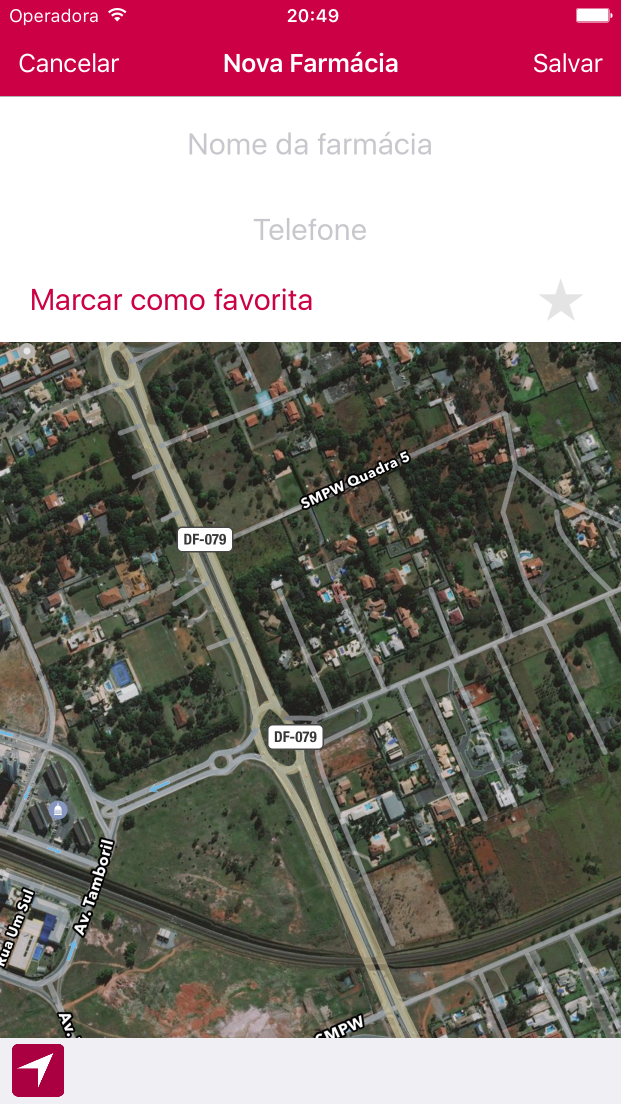
\includegraphics[width=0.9\linewidth]{ios_add_farma}
		\end{minipage}\hfill
		\begin{minipage}{.5\textwidth}
			\centering
			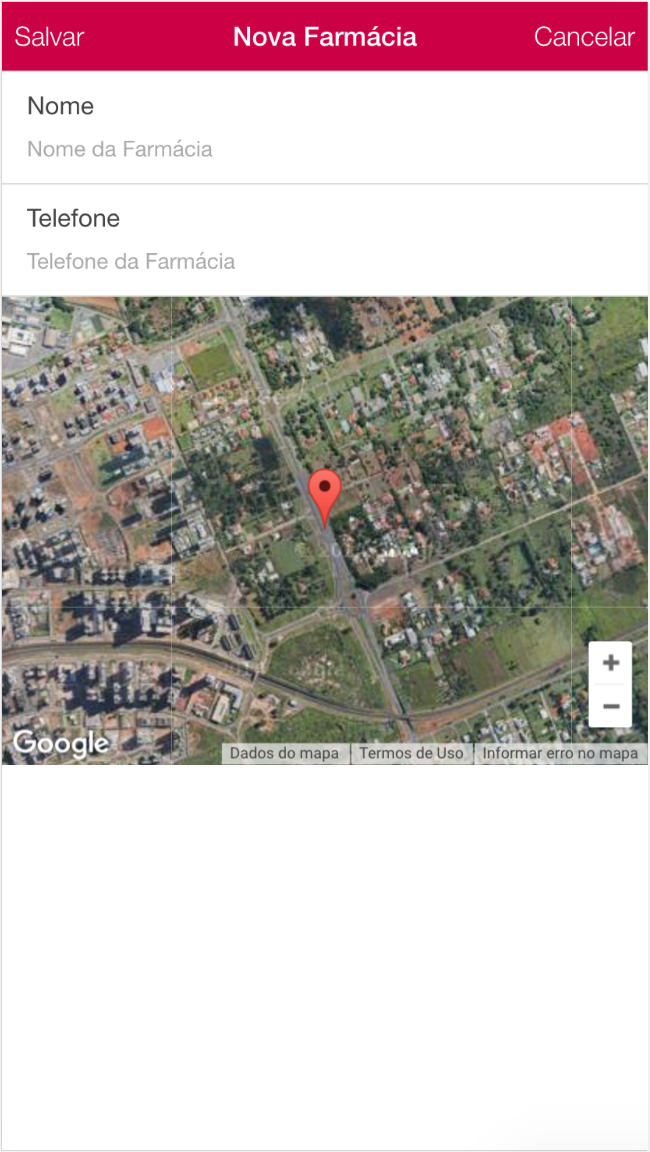
\includegraphics[width=0.9\linewidth]{ionic_add_farma}
		\end{minipage}
	\caption[Tela de adicionar farmácia (iOS \textit{versus} Ionic)]{ Tela de adicionar farmácia (iOS \textit{versus} Ionic). Fonte: Elaborado pelos autores.}
	\label{fig:add_farma}
	\end{figure}
 	
 	\item \textbf{Cadastro de Alertas};
 	
	\begin{itemize}
		\item Para o cadastro de um novo alerta, é preciso selecionar data e hora que o usuário será alertado. Para isso, o Ionic 1 não possui o componente adequado. Com isso, foi necessário procurar 
		e utilizar um \textit{framework} terceiro. Os \textit{frameworks} escolhidos foram o \textit{ionic-datepicker}\footnote{\url{https://github.com/rajeshwarpatlolla/ionic-datepicker}} e 
		\textit{ionic-timepicker}\footnote{\url{https://github.com/rajeshwarpatlolla/ionic-timepicker}}, respectivamente para seleção de data e hora. Ambos foram desenvolvidos pelo mesmo usuário no Github 
		e instalados no projeto do aplicativo via \textit{CLI}. Nas próprias documentações dos \textit{frameworks} existem exemplos de uso suficientes para guiar a implementação das funcionalidades. 
		Vale ressaltar que o componente do iOS possui a seleção de data e hora juntas, enquanto nos \textit{frameworks} utilizados, a seleção é separada, gerando uma pequena alteração na interface gráfica 
		da tela de cadastro de alertas quando comparada com a do aplicativo original. As diferenças entre o original e Ionic podem ser vistas na Figura~\ref{fig:dateTimePicker}. O mesmo \textit{framework}
		para seleção de data também foi utilizado na tela de cadastro de remédios para definir a data de validade do mesmo.

		\item Para a criação dos alertas é preciso cadastrar notificações locais na central de notificações do dispositivo. Realizar essa tarefa teve o mesmo nível de dificuldade da implementação no iOS nativo. 
		Apenas foi instalado um \textit{plugin} do Cordova para gerenciar a central de notificações e agendar notificações com as datas e horas corretas para serem entregues. 
	\end{itemize}

	\begin{figure}[H]
		\centering
		\begin{minipage}{.33\textwidth}
			\centering
			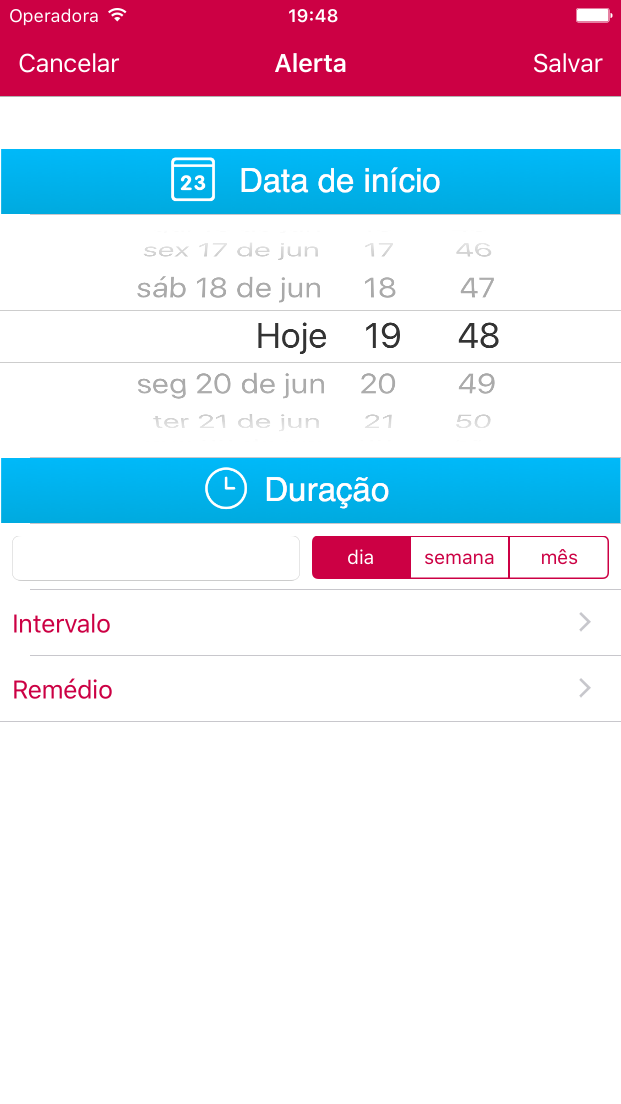
\includegraphics[width=0.95\linewidth]{ios_datetimepicker}
		\end{minipage}%
		\begin{minipage}{.33\textwidth}
			\centering
			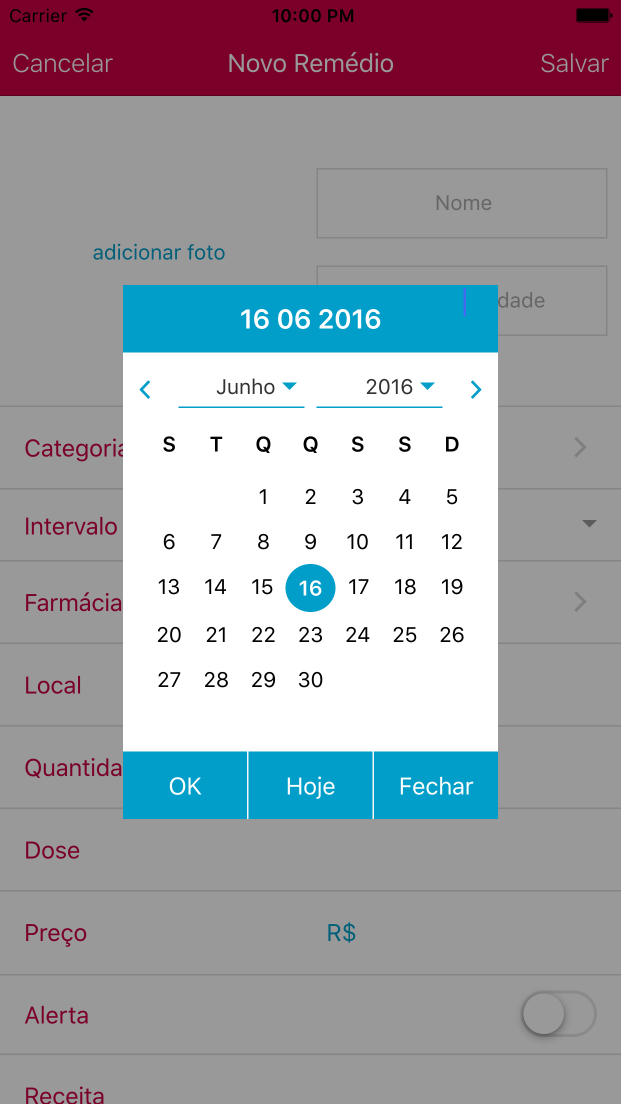
\includegraphics[width=0.95\linewidth]{ionic_datepicker}
		\end{minipage}
		\begin{minipage}{.33\textwidth}
			\centering
			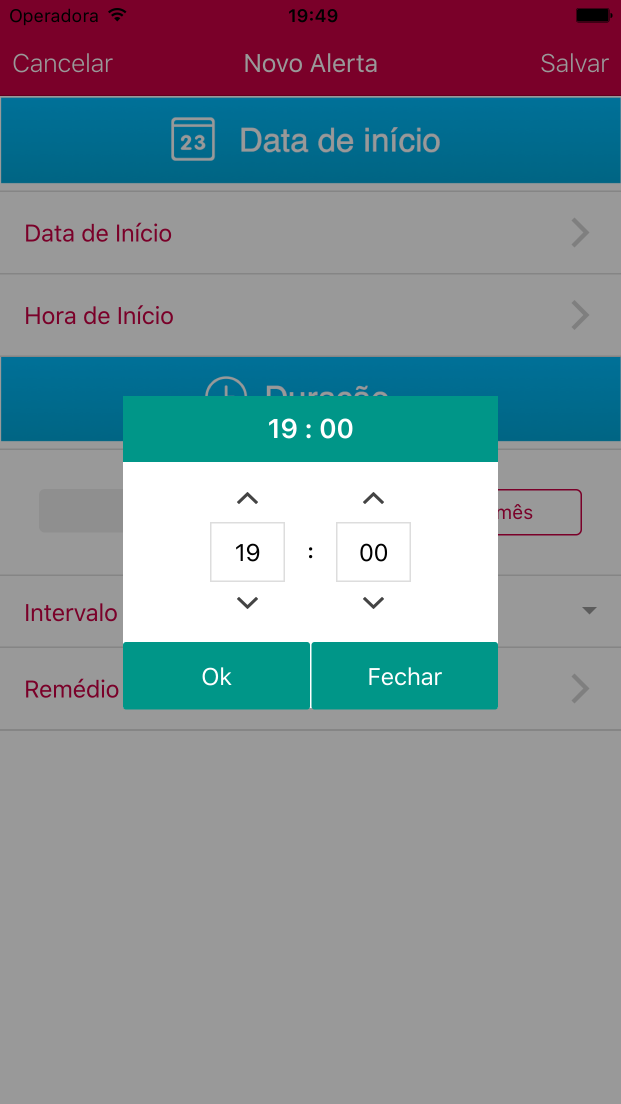
\includegraphics[width=0.95\linewidth]{ionic_timepicker}
		\end{minipage}
	\caption[Seleção de data e hora dos alertas (iOS \textit{versus} Ionic)]{ Seleção de data e hora dos alertas (iOS \textit{versus} Ionic). Fonte: Elaborado pelos autores.}
	\label{fig:dateTimePicker}
	\end{figure}
 	
 	\item \textbf{Observações gerais};
	\begin{itemize}
		\item Houve um problema para carregar a lista inicial de remédios, pois o Cordova não carrega as informações do banco de dados antes da \textit{view} terminar de ser carregada, o que 
		acarretava em falha na execução do aplicativo. Esse problema não existiu na criação do \textit{app} original e para contorná-lo foram feitas pesquisas na comunidade para saber como resolver.
		Umas das soluções era causar um \textit{delay} proposital no aplicativo para que desse tempo da \textit{view} ser carregada, mas foi descartada para não impactar negativamente na performance do
		\textit{app}. A solução utilizada foi fazer uma verificação a cada transação realizada no banco de dados para \textcolor{red}{verificar se o Ionic já carregou completamente ....}
		\item Não é possível debugar o aplicativo para iOS pelo terminal, assim como o Android, a partir da versão 9 do iOS.  
		Para tentar corrigir o problema, a documentação do Ionic sugere modificar uma configuração no arquivo \textit{.plist} do projeto iOS. No entanto, de acordo com relatos na internet e as próprias tentativas
		dos autores não foi possível obter sucesso. Com isso, para debugar é preciso de um computador com \textit{Xcode}, ou é possível também, utilizar os navegadores como \textit{Google Chrome} ou \textit{Safari}
		no modo desenvolvedor para debugar utilizando o console \textit{JavaScript} dos navegadores.
		\item Alguns erros do \textit{JavaScript} não são acusados pelo terminal do Ionic, dificultando a tarefa de \textit{debug} da aplicação. 
		Com isso, em um momento de dificuldade em achar um problema que estava acontecendo, algumas pesquisas foram realizadas na comunidade \textit{on-line} e em um fórum 
		de discussão sobre Ionic foi dada uma dica sobre o uso de alertas do \textit{JavaScript} para mostrar erros para o desenvolvedor e com isso facilitar na tarefa de debugar o aplicativo.
		\item A diretiva \textit{ng-class} do AngularJS não funciona em conjunto com a diretiva \textit{ion-nav} do Ionic. No entanto, isso não foi achado nas documentações, nem do Ionic e nem do AngularJS. 
		Novamente, recorremos à comunidade e foi dito que esses componentes não funcionam corretamente juntos.
		\item Por mais que os autores não possuissem conhecimentos avançados em \textit{HTML}, \textit{CSS} e \textit{JavaScript}, vale ressaltar que o conhecimento inicial nessas tecnologias ajudou muito 
		durante o desenvolvimento do \textit{app}, já que tudo é baseado nelas...
		\item O Cordova e o Ionic possuem documentações bem completas, apresentando exemplos de uso de códigos e as interfaces gráficas geradas com os códigos. A comunidade é ativa....
	\end{itemize}
 	
 	%\textcolor{red}{nao é possivel debugar o ios pelo terminal, por causa da atualizacao do ios 9, por isso é necessario do xcode ou do safari, ou seja um mac}

 	%\textcolor{red}{usar o banco na primeira controladora do sistema, cordova nao carrega antes da view}

 	%\textcolor{red}{possibilidade de debugar com os navegadores, é possivel usar os navegadores para poder debugar enquanto esta rodando no simulador das plataformas}

 	%\textcolor{red}{debug com alerta de javascript, nao eh falado em lugar nenhum, mas facilita muito. foi encontrado por pesquisas na comunidade on line}

 	%\textcolor{red}{ng-class nao funciona na ion-nav e foi muito dificil descobrir isso}

 	%\textcolor{red}{problemas na hora de executar no iphone, o projeto não executa corretamente as vezes por motivo desconhecido}

 	%- Site do cordova bem documentado, com exemplos de uso

 	%- Ressaltar a importancia de saber html, javascript e css
 \end{itemize} 



 \begin{figure}[H]
 	\centering
 	\begin{minipage}{.5\textwidth}
 		\centering
 		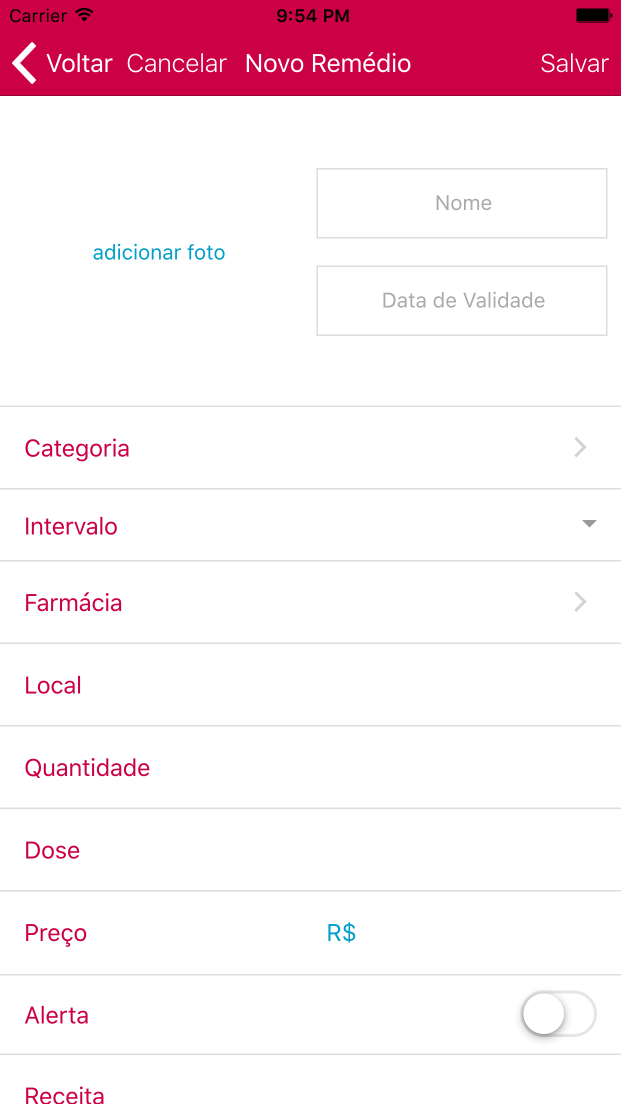
\includegraphics[width=.8\linewidth]{ionic_addremedio_ios}
 	\end{minipage}%
 	\begin{minipage}{.5\textwidth}
 		\centering
 		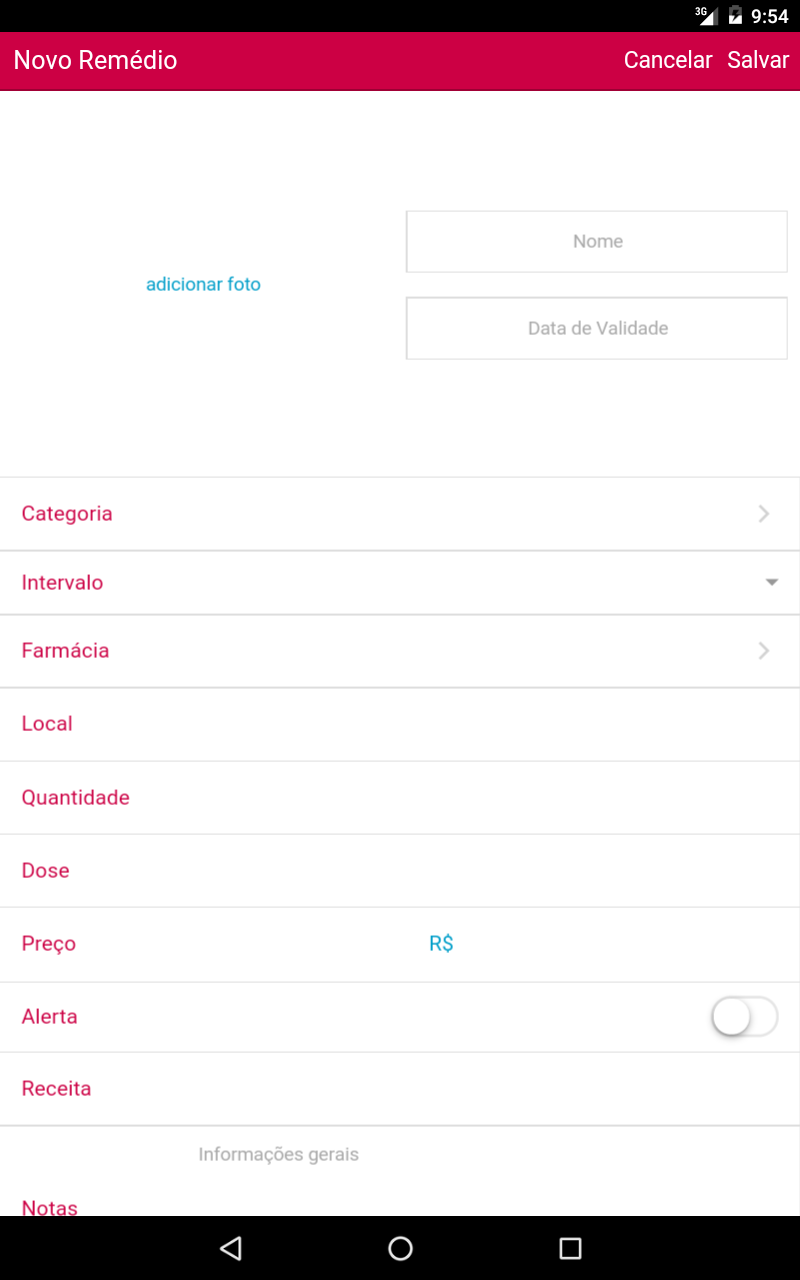
\includegraphics[width=0.9\linewidth]{ionic_addremedio_android}
 	\end{minipage}
 	\caption[Telas do cadastro de remédio (iOS \textit{versus} Android)]{ Telas do cadastro de remédio (iOS \textit{versus} Android). Fonte: Elaborado pelos autores.}
 	\label{fig:ionic_addremedio}
 \end{figure}